%%%%%%%%%%%%%%%%%%%%%%%%%%%%%%%%%%%%
% Slide options
%%%%%%%%%%%%%%%%%%%%%%%%%%%%%%%%%%%%

% Option 1: Slides with solutions

\documentclass[t,compress,mathserif]{beamer}
\newcommand{\soln}[1]{\textit{#1}}
\newcommand{\solnGr}[1]{#1}

% Option 2: Handouts without solutions

%\documentclass[11pt,containsverbatim,handout]{beamer}
%\usepackage{pgfpages}
%\pgfpagesuselayout{4 on 1}[letterpaper,landscape,border shrink=5mm]
%\newcommand{\soln}[1]{ }
%\newcommand{\solnGr}{ }


%%%%%%%%%%%%%%%%%%%%%%%%%%%%%%%%%%%%
% Style
%%%%%%%%%%%%%%%%%%%%%%%%%%%%%%%%%%%%

\def\chp5@path{../../Chp 5}
\input{../../lec_style.tex}

%%%%%%%%%%%%%%%%%%%%%%%%%%%%%%%%%%%%
% Preamble
%%%%%%%%%%%%%%%%%%%%%%%%%%%%%%%%%%%%

\title[Lecture 16]{MA213: Lecture 16}
\subtitle{Module 3: Foundations for inference}
\author{OpenIntro Statistics, 4th Edition}
\institute{$\:$ \\ {\footnotesize Based on slides developed by Mine \c{C}etinkaya-Rundel of OpenIntro. \\
The slides may be copied, edited, and/or shared via the \webLink{http://creativecommons.org/licenses/by-sa/3.0/us/}{CC BY-SA license.} \\
Some images may be included under fair use guidelines (educational purposes).}}
\date{}


%%%%%%%%%%%%%%%%%%%%%%%%%%%%%%%%%%%%
% Begin document
%%%%%%%%%%%%%%%%%%%%%%%%%%%%%%%%%%%%

\begin{document}

%%%%%%%%%%%%%%%%%%%%%%%%%%%%%%%%%%%%
% Title page
%%%%%%%%%%%%%%%%%%%%%%%%%%%%%%%%%%%%

{
\addtocounter{framenumber}{-1} 
{\removepagenumbers 
\usebackgroundtemplate{\includegraphics[width=\paperwidth]{../../OpenIntro_Grid_4_3-01.jpg}}
\begin{frame}

    \hfill \includegraphics[width=20mm]{../../oiLogo_highres}
    \titlepage

\end{frame}
}
}


%%%%%%%%%%%%%%%%%%%%%%%%%%%%%%%%%%%%
% Recap/Agenda 
%%%%%%%%%%%%%%%%%%%%%%%%%%%%%%%%%%%%
% TODO better formatting
\begin{frame}
    \frametitle{Module 3: Foundations for inference}
    \begin{itemize}
        \item \hl{Previously: }Point estimates and sampling variability (Chapter 5.1)
        \item \hl{This time: }Point estimates and sampling variability, continued (Chapter 5.1)
        \item \hl{Reading: }Chapter 5.2 for next time
        \item \hl{Deadlines/Announcements: }
        \begin{itemize}
            \item Reminder: Monday is a Holiday, Tuesday is Monday schedule
            \item Quiz 2 \hl{in class on Wednesday}, \textbf{Not in discussion sections}
            \item No discussion sections next week
        \end{itemize}
    \end{itemize}
    
\end{frame}
    
%%%%%%%%%%%%%%%%%%%%%%%%%%%%%%%%%%%%
% Learning objectives:
%%%%%%%%%%%%%%%%%%%%%%%%%%%%%%%%%%%%
\begin{frame}
\frametitle{Learning Objectives}
\begin{itemize}
    \item \textbf{M3 LO2: Visualize and Interpret Sampling Distributions:} Draw and interpret sampling distributions for a point estimate (e.g., population proportion) across different sample sizes, explaining how the distribution changes as the sample size increases. 
    \item \textbf{M3 LO3: Calculate and Interpret Standard Error:} Calculate the standard error for proportions and interpret it as a measure of sampling variability.
\end{itemize}
\end{frame}


%%%%%%%%%%%%%%%%%%%%%%%%%%%%%%%%%%%%
% Sections
%%%%%%%%%%%%%%%%%%%%%%%%%%%%%%%%%%%%

\section{Sampling distributions}

\begin{frame}
    \frametitle{}
    
    \dq{Suppose that you don't have access to the population of all American adults, which is a quite likely scenario. In order to estimate the proportion of American adults who support solar power expansion, you might sample from the population and use your sample proportion as the best guess for the unknown population proportion.}
    
    \begin{itemize}
    
    \item Sample 1000 American adults from the population, and record whether they support or not solar power expansion.
    
    \item Find the sample proportion.
    
    \item Repeat this process many times and plot the distribution of the sample proportions obtained by this experimental design.
    
    \end{itemize}
    
A \hl{Sampling Distribution} is the distribution of a \hl{statistic} (any function of the data, e.g., sample proportion), where the randomness comes from sampling randomly from a population.
\end{frame}
%%%%%%%%%%%%%%%%%%%%%%%%%%%%%%%%%%%%

\begin{frame}
    \frametitle{Edfinity Quiz}
    \begin{center}
        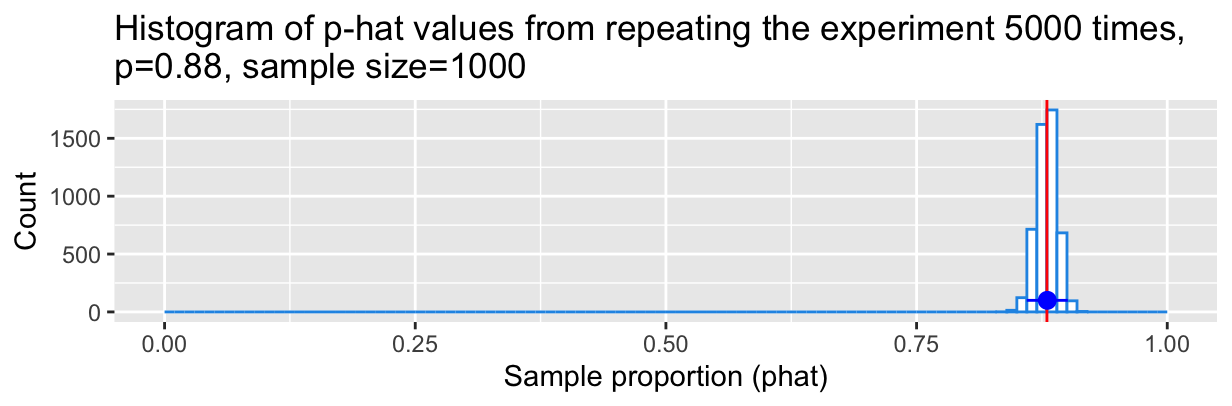
\includegraphics[width=0.75\textwidth]{../Lecture15/sampling_distribution.png}
    \end{center}
    
    \soln{
    \begin{table}[h!]
        \centering
        \begin{tabular}{|c|c|c|c|}
        \hline
         & Middle? & Symm? & Wider/Narrower/Same? \\ 
        \hline
        p=0.88, n=1000 & $\sim0.88$ & Yes & Same \\ 
        \hline
        p=0.5, n=100 & $\sim0.5$ & Yes & Wider \\ 
        \hline
        p=0.99, n=100 & $\sim0.99$ & No & Same? \\ 
        \hline
        \end{tabular}
    \end{table}
    }
\end{frame}

%%%%%%%%%%%%%%%%%%%%%%%%%%%%%%%%%%%%

\begin{frame}
    \frametitle{Edfinity Quiz}
    What would happen if the sample size were 10?
\end{frame}

%%%%%%%%%%%%%%%%%%%%%%%%%%%%%%%%%%%%

%%%%%%%%%%%%%%%%%%%%%%%%%%%%%%%%%%

\section{R Demo: What would happen if...}

%%%%%%%%%%%%%%%%%%%%%%%%%%%%%%%%

\begin{frame}
\frametitle{Sampling distribution of the sample proportion}
    \begin{itemize}
        \item For a sample of size $n$ and population proportion $p$, the number of successes $X \sim \text{Binomial}(n, p)$
        \item The sample proportion is a rescaled version of $X$: $\hat{p} = \frac{X}{n}$
        \item So the sampling distribution of $\hat{p}$ is just like the binomial distribution, but for values from $0$ to $1$ instead of $0$ to $n$
    \end{itemize}
    \vspace{2em}
    \begin{columns}[T] 
        \begin{column}{0.4\textwidth}
            \vspace{2em} 
            \footnotesize{\textcolor{red}{Note:} Assumes that the population is much larger than the sample, so that sampling with replacement is a good approximation to sampling without replacement.}
        \end{column}
        \begin{column}{0.6\textwidth}
            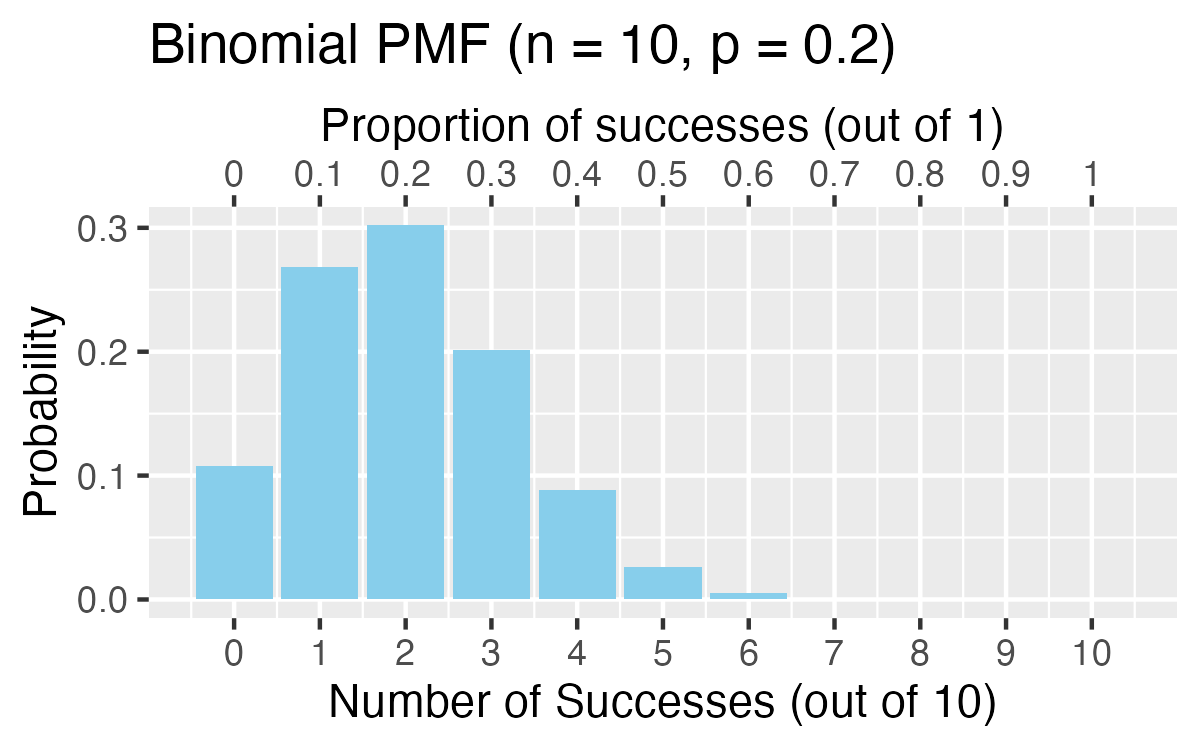
\includegraphics[width=\textwidth]{sampling_dist_of_phat.png}
        \end{column}
    \end{columns}
\end{frame}

%%%%%%%%%%%%%%%%%%%%%%%%%%%%%%%%%%%

\begin{frame}
\frametitle{Sampling distribution of the sample proportion}

$X \sim \text{Binomial}(n, p)$ \\
$\hat{p}  = \frac{X}{n}$ \\
\pause
\vspace{1em}
\textcolor{orange}{$Pr(\hat{p}  = \frac{k}{n}) = Pr(X = k) = \dbinom{n}{k} p^k (1-p)^{n-k}$} \\
for $\frac{k}{n} \in \left\{0, \frac{1}{n}, \frac{2}{n}, \ldots, \frac{n-1}{n}, 1\right\}$
\pause

This is the theoretical \hl{sampling distribution} of $\hat{p}$!
\end{frame}
%%%%%%%%%%%%%%%%%%%%%%%%%%%%%%%%%%

\section{Edfinity quiz}

%%%%%%%%%%%%%%%%%%%%%%%%%%%%%%%%%%%

\begin{frame}
\frametitle{Sampling distribution of the sample proportion}

$X \sim \text{Binomial}(n, p)$ \\
$\hat{p}  = \frac{X}{n}$ \\

\vspace{1em}
\textcolor{orange}{$Pr(\hat{p}  = \frac{k}{n}) = Pr(X = k) = \dbinom{n}{k} p^k (1-p)^{n-k}$} \\
for $\frac{k}{n} \in \left\{0, \frac{1}{n}, \frac{2}{n}, \ldots, \frac{n-1}{n}, 1\right\}$


This is the theoretical \hl{sampling distribution} of $\hat{p}$!
\vspace{1em}

\soln{
$E[\hat{p}] = \frac{1}{n}E[X] = \frac{1}{n}np = p$\\
$Var[\hat{p}] = \frac{1}{n^2}Var[X] = \frac{1}{n^2}np(1-p) = \frac{p(1-p)}{n}$
}
\pause

\vspace{1em}
The \hl{Standard Error} is the standard deviation of the sampling distribution. Here, $SE_{\hat{p}} = \sqrt{\frac{p(1-p)}{n}}$
\end{frame}
%%%%%%%%%%%%%%%%%%%%%%%%%%%%%%%%%%

\begin{frame}
\frametitle{What we just did is profound!}
\begin{itemize}
    \item We modeled the sample proportion (a data summary statistic) using our tools from probability (the Binomial distribution).
    \pause
    \item Using this model, we wrote down the \emph{theoretical} sampling distribution of the sample proportion $\hat{p}$ \\
    (not just a simulated sampling distribution).
    \pause
    \item We used the rules for linear combinations of random variables to derive the mean and variance of the sampling distribution.
    \pause
    \item We can use these results to evaluate the quality of $\hat{p}$ as an estimator for $p$:
    \begin{itemize}
        \item $\hat{p}$ is an \hl{unbiased} estimator for $p$ since $E[\hat{p}] = p$
        \item The standard error $SE_{\hat{p}} = \sqrt{\frac{p(1-p)}{n}}$ gets smaller as $n$ increases, so larger samples give more consistent estimates of $p$.
    \end{itemize}
\end{itemize}
\end{frame}

%%%%%%%%%%%%%%%%%%%%%%%%%%%%%%%%%%%%

\section{Different estimators for the same parameter}

%%%%%%%%%%%%%%%%%%%%%%%%%%%%%%%%%

\begin{frame}
    \frametitle{Rule of succession}

    There can be multiple statistics that estimate the same population parameter
    \begin{itemize}

        \item \hl{The Rule Of Succession} (Laplace, 18th Century)
        \item What is the probability that the sun will rise tomorrow, given that it has risen every day for the last 5000 years?
        \item 0 is an unsatisfying answer
        \item Approach: Pretend we have seen one success and one failure
    
    \end{itemize}

    Sample proportion:
     \begin{align}
        \hat{p}=\frac{X}{n}
    \end{align}
 
    Rule of Succession:
    \begin{align}
        \hat{p}^*=\frac{X +1}{n+2}
    \end{align}
 
\end{frame}


%%%%%%%%%%%%%%%%%%%%%%%%%%%%%%%%%%%%

\section{R Demo: Comparing different estimators based on their sampling distributions}

%%%%%%%%%%%%%%%%%%%%%%%%%%%%%%%%%%
\begin{frame}
    \frametitle{Comparing different estimators based on their sampling distributions}

    \begin{itemize}
        \item We can use simulations to compare different estimators for the same population parameter
        \item In general, we want an estimator that
        \begin{itemize}
            \item is unbiased, i.e. the mean of the sampling distribution is equal to the population parameter
            \item has low variability, i.e. the standard error is small
        \end{itemize}
        \item But sometimes it is helpful to have some bias for small samples, as long as the bias goes away for large samples (e.g. the rule of succession)
        \item And often, there is a trade-off between bias and variability
    \end{itemize}
\end{frame}

%%%%%%%%%%%%%%%%%%%%%%%%%%%%%%%%

\section{Sampling distribution for the sample mean of a Normal population}

\begin{frame}
\frametitle{Sampling distribution for the sample mean of a Normal population}
\begin{itemize}
    \item So far we've studied estimators for population proportions
    \item We can also use the same framework to study estimators for population means
\end{itemize}
If the population is Normal with mean $\mu$ and standard deviation $\sigma$, what is the sampling distribution of the sample mean $\bar{X}$?
\end{frame}

%%%%%%%%%%%%%%%%%%%%%%%%%%%%%%%%%%%
\begin{frame}
\frametitle{Sampling distribution for the sample mean}
Let $X_1, X_2, \ldots, X_n$ be an iid random sample where $X_i \sim Normal(\mu, \sigma)$

What is the distribution of: 
\begin{align}
    \bar{X}=\frac{1}{n}(X_1 + X_2 + \ldots + X_n)=\frac{1}{n}\sum_{i=1}^{n} X_i
\end{align}
\pause 

It turns out that linear combinations of independent Normal random variables are also Normal

So: \textcolor{orange}{
$\bar{X}\sim Normal\left(\mu_{\bar{X}}, \sigma_{\bar{X}}\right)$
}
for some $\mu_{\bar{X}}$ and $\sigma_{\bar{X}}$. What are they?

\pause
We already solved this in Lecture 9!

\end{frame}

%%%%%%%%%%%%%%%%%%%%%%%%%%%%%%%%
\begin{frame}
\frametitle{Pair work from Lecture 9}
\dq{Given an independent sample $X_1, X_2, \ldots, X_n$, where $E[X_i]=\mu$ and $Var[X_i]=\sigma^2$. 

The sample mean is defined as:

\begin{center}$\bar{X}=\frac{1}{n}\left(X_1 + X_2 + \ldots + X_n\right)=\frac{1}{n}\sum_{1}^{n} X_i$\end{center}

What is $E[\bar{X}]$? What is $Var[\bar{X}]$? What is $StdDev[\bar{X}]$?}

\begin{eqnarray*} 
E[\bar{X}] &=& E\left[\frac{1}{n}\sum_{i=1}^{n} X_i\right] = \frac{1}{n}\sum_{i=1}^{n} E[X_i] = \frac{1}{n}\times n \times \mu = \mu \\
\pause
Var[\bar{X}] &=& Var\left[\frac{1}{n}\sum_{i=1}^{n} X_i\right] = \frac{1}{n^2}\sum_{i=1}^{n} Var[X_i] = \frac{1}{n^2}\times n \times \sigma^2 = \frac{\sigma^2}{n} \\
StdDev[\bar{X}] &=& \sqrt{\frac{\sigma^2}{n}} = \frac{\sigma}{\sqrt{n}}
\end{eqnarray*} 

\end{frame}
%%%%%%%%%%%%%%%%%%%%%%%%%%%%%%%%

\begin{frame}
\frametitle{Sampling distribution for the sample mean of a Normal population}
Let $X_1, X_2, \ldots, X_n$ be an iid random sample where $X_i \sim Normal(\mu, \sigma)$

What is the distribution of: 
\begin{align}
    \bar{X}=\frac{1}{n}(X_1 + X_2 + \ldots + X_n)=\frac{1}{n}\sum_{i=1}^{n} X_i
\end{align}
\textcolor{orange}{
\begin{align*}
 \bar{X} &\sim Normal\left(\mu_{\bar{X}}=\mu, \sigma_{\bar{X}}=\frac{\sigma}{\sqrt{n}}\right)
\end{align*}
}
\end{frame}

%%%%%%%%%%%%%%%%%%%%%%%%%%%%%%%%

\section{Edfinity quiz}

%%%%%%%%%%%%%%%%%%%%%%%%%%%%%%%%%
\begin{frame}
\frametitle{Quality of the sample mean as an estimator for the population mean}
\textcolor{orange}{
\begin{align*}
 \bar{X} &\sim Normal\left(\mu_{\bar{X}}=\mu, \sigma_{\bar{X}}=\frac{\sigma}{\sqrt{n}}\right)
\end{align*}
}
\dq{What does this tell us about the quality of $\bar{X}$ as an estimator for $\mu$?}
\soln{
The sample mean is an \hl{unbiased} estimator for the population mean, and the standard error (standard deviation of the sampling distribution) gets smaller with the square root of the sample size}

\end{frame}
%%%%%%%%%%%%%%%%%%%%%%%%%%%%%%%%

\section{Central Limit Theorem (Ch. 5.1-5.2)}

%%%%%%%%%%%%%%%%%%%%%%%%%%%%%%%%%%%%

\section{R Demo: For large samples, does the sample proportion also have a Normal sampling distribution? }

%%%%%%%%%%%%%%%%%%%%%%%%%%%%%%%%%

\begin{frame}
\frametitle{Central Limit Theorem}

\formula{Central limit theorem (sample proportion)}
{Sample proportions will be nearly normally distributed with mean equal to the population proportion, $p$, and standard error equal to $\sqrt{\frac{p~(1-p)}{n}}$.
\[ \hat{p} \sim N \pr{ mean = p, SE = \sqrt{\frac{p~(1-p)}{n}} } \]
}

\begin{itemize}

\item This comes from the fact that the Binomial distribution converges to the Normal distribution as $n$ increases.
\item The standard error $SE =  \sqrt{\frac{p~(1-p)}{n}}$ is what we derived on the board for $\hat{p}$. Note that as $n$ increases $SE$ decreases.
\begin{itemize}
\item As $n$ increases samples will yield more consistent $\hat{p}$s, i.e. variability among $\hat{p}$s will be lower.
\end{itemize}

\end{itemize}

\end{frame}

%%%%%%%%%%%%%%%%%%%%%%%%%%%%%%%%%%%%

\begin{frame}
\frametitle{CLT - conditions}

Certain conditions must be met for the CLT to apply:

\begin{enumerate}

\item \hlGr{Independence:} Sampled observations must be independent. \\

This is difficult to verify, but is more likely if
\begin{itemize}
\item random sampling/assignment is used, and
\item if sampling without replacement, $n$ $<$ 10\% of the population.
\end{itemize}

\pause

\item \hlGr{Sample size:} There should be at least 10 expected successes and 10 expected failures in the observed sample.

This is difficult to verify if you don't know the population proportion (or can't assume a value for it). In those cases we look for the number of observed successes and failures to be at least 10.

\end{enumerate}

\end{frame}

%%%%%%%%%%%%%%%%%%%%%%%%%%%%%%%%%%

\begin{frame}
\frametitle{When the conditions are not met...}

\begin{itemize}

\item When either $np$ or $n(1-p)$ is small, the distribution is more discrete.
\item When $np$ or $n(1-p)$ $<$ 10, the distribution is more skewed.
\item The larger both $np$ and $n(1-p)$, the more normal the distribution.
\item When $np$ and $n(1-p)$ are both very large, the discreteness of the distribution is hardly evident, and the distribution looks much more like a normal distribution.

\end{itemize}

\end{frame}

%%%%%%%%%%%%%%%%%%%%%%%%%%%%%%%%

\begin{frame}
\frametitle{CLT for the sample mean}

\formula{Central limit theorem (sample mean)}
{Sample means will be nearly normally distributed with mean equal to the population mean, $\mu$, and standard error equal to $\frac{\sigma}{\sqrt{n}}$.
\[ \bar{X} \sim N \pr{ mean = \mu, SE = \frac{\sigma}{\sqrt{n}} } \]
}

\begin{itemize}
    \item This is exactly true if the population distribution is Normal, regardless of sample size $n$ (we derived this earlier)
    \item But it is also true \emph{regardless of the shape of the population distribution}, as long as the sample size $n$ is sufficiently large.
    \item Different distributions will require different sample sizes for the CLT to ``kick in''.
    \item This is the topic of Lab 5, and we will revisit it in more detail in Chapter 7.
\end{itemize}

\end{frame}
%%%%%%%%%%%%%%%%%%%%%%%%%%%%%%%%%%%%

%%%%%%%%%%%%%%%%%%%%%%%%%%%%%%%%%%%%

\subsection{Extending the framework for other statistics}

%%%%%%%%%%%%%%%%%%%%%%%%%%%%%%%%%%%%

\begin{frame}
\frametitle{Extending the framework for other statistics}

\begin{itemize}

\item The strategy of using a sample statistic to estimate a parameter is quite common, and it's a strategy that we can apply to other statistics besides a proportion or a mean.

\item The principles and general ideas from this chapter apply to other parameters as well, even if the details change a little. 
\begin{itemize}
    \item Using statistics (functions of data) to estimate parameters (population values)
    \item Modeling the sampling process and the statistic using probability tools
    \item Deriving or Simulating the sampling distribution of the statistic
    \item Evaluating bias (is the mean of the sampling distribution equal to the parameter?)
    \item Evaluating variability (how does the standard error change with sample size?)
\end{itemize}
\end{itemize}
\end{frame}

%%%%%%%%%%%%%%%%%%%%%%%%%%%%%%%%%%%%
% End document
%%%%%%%%%%%%%%%%%%%%%%%%%%%%%%%%%%%%

\end{document}